\section{Evaluation}
\label{sec:eval}

%TODO: Add a scalable column to table
%% constructs to cover:
%% filter, map, zip, groupby
%% with and without emits
%% show composition
%% show headers as well as performance metadata conditions

\begin{table*}[!t]
\centering
\resizebox{\textwidth}{!}{%
\begin{tabular}{llllllll}
\hline

{\textbf{Example}} &
{\textbf{Query code}} &
{\textbf{Description}} &
{\textbf{Linear}} &
{\textbf{Scales?}} &
{\textbf{Pipe}} &
{\textbf{Pipe}} & 
{\textbf{\# of}} \\

&
&
&
{\textbf{in state?}} &
&
{\textbf{depth}} &
{\textbf{width}} &
{\textbf{atoms}} \\

\hline
\hline

Packet counts &
{\ct def count([cnt], []): cnt = cnt + 1; emit() } &
Count packets per source IP. &
Yes &
Yes &
5 &
2 &
7 \\

&
{\ct result = groupby(\pktlog, [srcip], count);} &
&
&
&
&
&
\\

\hline

EWMA over latencies &
{\ct def ewma([avg], [tin, tout]):} &
Maintain a moving EWMA over &
Yes &
Yes &
6 &
4 &
11 \\

&
{\ct \ \ avg = (1-alpha)*avg + (alpha)*(tout-tin)} &
packet latencies per flow. &
&
&
&
\\

&
{\ct ewma\_q = groupby(\pktlog, [\codeftuple{}], ewma);} &
&
&
&
&
\\

\hline

TCP out-of-sequence &
{\ct def oos([lastseq, cnt], [tcpseq, payload\_len]):} &
Count the number of packets per &
Yes &
Yes &
7 &
4 & 
14 \\

&
{\ct \ \ if lastseq != tcpseq: cnt = cnt + 1} &
connection arriving with a sequence &
&
&
&
\\

&
{\ct \ \ lastseq = tcpseq + payload\_len } &
number that is non-consecutive with &
&
&
&
\\

&
{\ct oos\_q = groupby(\pktlog, [\codeftuple{}], oos);} &
the last packet. &
&
&
&
\\

\hline

TCP non-monotonic &
{\ct def nonmt([maxseq, cnt], [tcpseq]):} &
Count the number of packets per &
No &
No &
5 &
2 &
6 \\

&
{\ct \ \ if maxseq > tcpseq: cnt = cnt + 1} &
connection with sequence numbers &
&
&
&
\\

&
{\ct \ \ else: maxseq = tcpseq} &
lower than the maximum so far. &
&
&
&
\\

&
{\ct nm\_q = groupby(\pktlog, [\codeftuple{}], nonmt);} &
&
&
&
&
\\

\hline

Flowlet size &
{\ct def fl\_detect([last\_time, size], [tin]):} &
Compute a histogram over the &
Yes &
No &
11 &
6 & 
31 \\

histogram &
{\ct \ \ if tin - last\_time > delta:} &
lengths of flowlets. This statistic is &
&
&
&
\\

&
{\ct \ \ \ \ emit(); size = 1 } &
 useful to evaluate network load &
&
&
&
\\

&
{\ct \ \ else: size = size + 1} &
balancing schemes, \eg\cite{conga}. &
&
&
&
\\

&
{\ct \ \ last\_time = tin} &
&
&
&
&
\\

&
{\ct R1 = groupby(\pktlog, [\codeftuple{}], fl\_detect);} &
&
&
&
&
\\

&
{\ct fl\_hist = groupby(R1, [size], count);} &
&
&
&
&
\\

\hline

High E2E latency &
{\ct def sum\_lat([e2e\_lat], [tin, tout]): } &
Capture packets experiencing high &
Yes &
Yes &
5 &
3 &
8 \\

&
{\ct \ \ e2e\_lat = e2e\_lat + tout - tin} &
end-to-end queueing latency, by &
&
&
&
\\

&
{\ct e2e = groupby(\pktlog, [uid], sum\_lat);} &
adding time spent in the queue at &
&
&
&
\\

&
{\ct high\_e2e = filter(e2e, e2e\_lat > 10);} &
each hop. &
&
&
&
\\

\hline

Count concurrently &
{\ct def new\_flow([cnt], []):} &
Count the number of active &
No &
No &
4 &
3 & 
10 \\

active connections &
{\ct \ \ if cnt == 0: emit(); cnt = 1} &
connections in a queue over a &
&
&
&
\\

&
{\ct R1 = map(\pktlog, [tin/128], [epoch]);} &
period of time (``epoch''). &
&
&
&
\\

&
{\ct R2 = groupby(R1, [\codeftuple, epoch], new\_flow);} &
&
&
&
&
\\

&
{\ct num\_conns = groupby(R2, [epoch], count);} &
&
&
&
&
\\

\hline

TCP incast &
{\ct R3 = zip(num\_conns, \pktlog);} &
Detect when many connections use &
No &
No &
7 &
4 &
14 \\

&
{\ct ic\_q = filter(R3, qin > 100 and cnt < 25);} &
a long queue. Uses the query above. &
&
&
&
\\

%&
%{\ct } &
%queue. Builds on the query above. &
%&
%&
%&
%\\

\hline

Lossy connections &
{\ct total = groupby(\pktlog, [\codeftuple{}], count);} &
Compute packet loss rate per &
Yes &
No &
8 &
4 &
19 \\

&
{\ct R1 = filter(\pktlog, tout == infinity);} &
connection, reporting connections &
&
&
&
\\

&
{\ct lost = groupby(R1, [\codeftuple{}], count);} &
with packet drop rate higher than &
&
&
&
\\

&
{\ct Z = zip(total, lost);} &
a threshold {\ct p.} &
&
&
&
\\

&
{\ct lc\_q = filter(Z, lost.cnt > p*total.cnt);}
&
&
&
&
\\

\hline

TCP timeouts &
{\ct def timeout([cnt], [last\_time, tin]):} &
Count the number of timeouts for &
Yes &
Yes &
8 &
3 &
15 \\

&
{\ct \ \ timediff = tin - last\_time } &
each TCP connection, by checking &
&
&
&
\\

&
{\ct \ \ if timediff > 280ms and timediff < 320ms:} &
for packet inter-arrival times &
&
&
&
\\

&
{\ct \ \ \ \ cnt = cnt + 1} &
around 300 ms (retransmission &
&
&
&
\\

&
{\ct \ \ last\_time = tin} &
timer). &
&
&
&
\\

&
{\ct to\_q = groupby(\pktlog, [\codeftuple{}], timeout);} &
&
&
&
&
\\

\hline

%% %% template left behind to create new rows quickly
%% &
%% {\ct } &
%% &
%% \\

\end{tabular}
}
\caption{Examples of performance queries. We
report that a query {\em scales} to a large number of keys either if (1) there
are no stateful updates involved, or (2) all its stateful updates are
linear-in-state {\em and} there are no {\ct emit()}s. We use
Domino~\cite{domino_sigcomm} to report the hardware resources, \ie atom count and pipeline depth and width. Linear-in-state queries use the
multiply-accumulate atom (\Sec{aggregation}); others use a NestedIf
atom~\cite{domino_sigcomm} that supports updates predicated on the state value
itself.}
\vspace{-0.1in}
%
%We label the query
%{\em linear-in-state} if all its stateful updates are linear-in-state. 
\label{tab:example-perf-queries}
\end{table*}

%The performance of Marple in practice depends on three factors: hardware feasibility, result accuracy, and ease of use.
%Section~\ref{s:eval:hardware} discusses the required hardware atoms required to perform aggregations at line rate. We show that Marple's silicon requirements are modest and realizable with current technology.
%Section~\ref{s:eval:traces} presents a Marple aggregation run on traces of both core Internet and datacenter traffic, to demonstrate how the size of the in-memory key-value store affects the number of flows Marple can accurately track.
%Finally, Section~\ref{s:eval:mininet} presents a case study using Marple to
%diagnose the root cause of irregular HTTP traffic.

We evaluate \TheSystem along three dimensions. In \Sec{eval:hardware}, we show
the router compute resources used for some candidate \TheSystem queries, while
in \Sec{eval:traces}, we measure the memory-bandwidth tradeoff for the
key-value store. In \Sec{eval:mininet}, we show an end to end use case of
\TheSystem by debugging a performance problem, {\em microbursts,} on the P4
behavioral model.

\subsection{Hardware compute resources}
\label{s:eval:hardware}
\label{sec:eval:hardware}

Table~\ref{tab:example-perf-queries} shows several \TheSystem queries.  Next to
each query, we show (1) whether all its aggregations are linear-in-state, (2)
whether it can be scaled by merging correctly with a backing store, and (3) the
router resources required, measured through the pipeline depth (number of
stages), pipeline width (maximum number of parallel computations per stage),
and the number of Banzai atoms (total number of computations).

Table~\ref{tab:example-perf-queries} shows that many useful queries contain
only linear-in-state aggregations, and many of them can be implemented scalably
(\Sec{linear-in-state-description}). Notably, the flowlet size histogram and
lossy connection queries are not scalable despite being linear-in-state, since
they contain {\ct emit()} statements.  In \Sec{workaround-nonscalable}, we
showed how to rewrite some of these queries (\eg lossy connections) to scale,
at the cost of losing some accuracy.

We compute the pipeline's depth and width by compiling each query to Banzai
using the Domino compiler. When compiling each query, Banzai is supplied with a
single stateless atom type, which perform binary operations (arithmetic, logic,
and relational) on pairs of packet fields, and a stateful atom type depending
on the type of the query.  For the linear-in-state queries, we use the
multiply-accumulate atom as the stateful atom, while for the other operations,
we use the NestedIf atom (Table~\ref{tab:templates}). As expected, all the
linear-in-state queries compile to a pipeline with the multiply-accumulate
atom; for all the queries that are not linear-in-state, the NestedIf atom turns
out to be sufficiently expressive.

The computational resources required for \TheSystem queries are modest.  All
queries in Table~\ref{tab:example-perf-queries} require a pipeline shorter than
11 stages.  This is feasible, \eg the RMT architecture offers 32
stages~\cite{rmt}. Further, functionality other than measurement can run in
parallel in each stage because the number of atoms required per stage is at
most 6, while programmable routers provide a few 100 parallel instructions per
stage (\eg RMT provides 224~\cite{rmt}).

\subsection{Memory and Bandwidth Overheads}
\label{s:eval:traces}
\label{sec:eval:traces}

%% The details of the on-chip cache
%% and backing store depend on the type traffic that passes through the switch.

In this section, we evaluate our key-value store design by running \TheSystem on
traces from both core Internet and data center switches to answer the following
questions:
\begin{CompactEnumerate}
\item What is a good size for the on-chip key value store?
\item How to equip the backing store to handle evictions?
\item How accurate are queries that aren't mergeable?
%%   What throughput should the backing store support?
%% \item What is the accuracy for queries not linear in state?
\end{CompactEnumerate}

\Para{Setup.}  We simulate a \TheSystem aggregation to count the number of
packets per \txtftuple over three separate {\em non-sampled} traces: two
five-minute traces from core Internet switches, one from Chicago
(\textasciitilde{}150 million packets) in April 2016~\cite{caida2016} and one
from San Jose (\textasciitilde{}189 million packets) in June
2014~\cite{caida2014}; and a 2.5 hour university datacenter trace
(\textasciitilde{}100 million packets) from 2010~\cite{bensonDC}. We refer to
these traces as Core16, Core14, and DC, respectively.

The aggregation key (a \txtftuple) requires 104 bits, and we assume a 24-bit
counter value, which totals 128 bits per entry in the key-value store. As
discussed in \Sec{hardware-feasibility}, our hardware design uses an 8-way LRU
cache. However, we also evaluate two other geometries: a hash table, which
evicts the incumbent key upon a collision, and a fully associative LRU
cache. Comparing our 8-way LRU with other hardware designs lets us evaluate the
tradeoff between hardware complexity, memory, accuracy, and eviction rate.

Based on an analysis of the traces, we use an average packet size of 700 bytes
and a network utilization of 30\%, to translate the number of evictions in our
results to an eviction rate (in packets per second) for a switch processing one
billion 64-byte packets per second.

\Para{On-chip cache size}.  The on-chip cache size significantly impacts the
eviction rate for mergeable queries, and the accuracy for queries that are not
mergeable. A larger cache causes fewer evictions---and hence a smaller load---on
the backing store. For non-mergeable aggregations, fewer evictions also produces
a higher accuracy. However, a larger cache size demands a larger silicon die
area and is more costly to manufacture.

Current SRAM densities are
$\approx7000\nicefrac{Kb}{mm^2}$~\cite{sram_estimate}, and the smallest
switching chips occupy 200 \si{\milli\metre\squared}~\cite{gibb_parsing}.
Therefore, a 32-Mbit cache in SRAM costs under 2.5\% additional area, which we believe is a reasonable overhead. Our trace-driven simulations thus target a 32-Mbit cache, while testing
a range from 8 Mbits ($2^{16}$ pairs) to 256 Mbits ($2^{21}$ pairs).

\Para{Eviction Rate.} Each key-value pair evicted from the switch must be streamed to a backing store.
This requires the backing store to be able to process packets at the eviction rate. We measure the eviction rates over (a) the 3 traces using the 8-way LRU geometry (\Fig{eviction-traces}) and (b) the three geometries for the DC trace (\Fig{eviction-geo}).
\begin{figure}[ht]
\centering
\vspace{-0.1in}
\begin{subfigure}[t]{0.48\columnwidth}
\raggedright
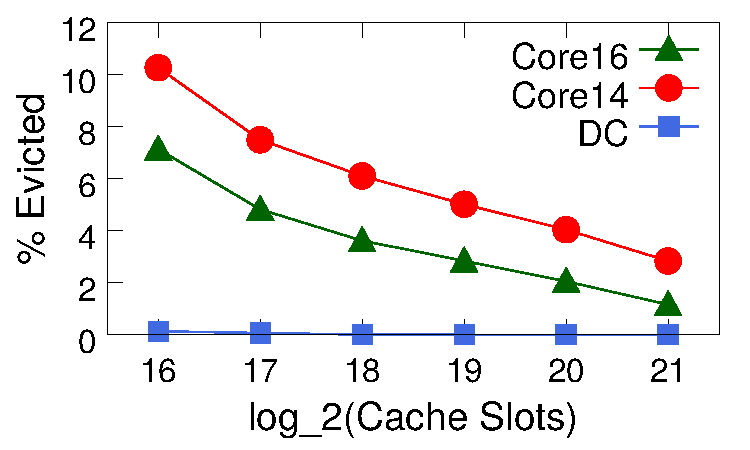
\includegraphics[width=\linewidth]{pq_eviction-rate-alltraces.pdf}
\caption{By trace}
\label{fig:eviction-traces}
\end{subfigure}
\begin{subfigure}[t]{0.48\columnwidth}
\raggedleft
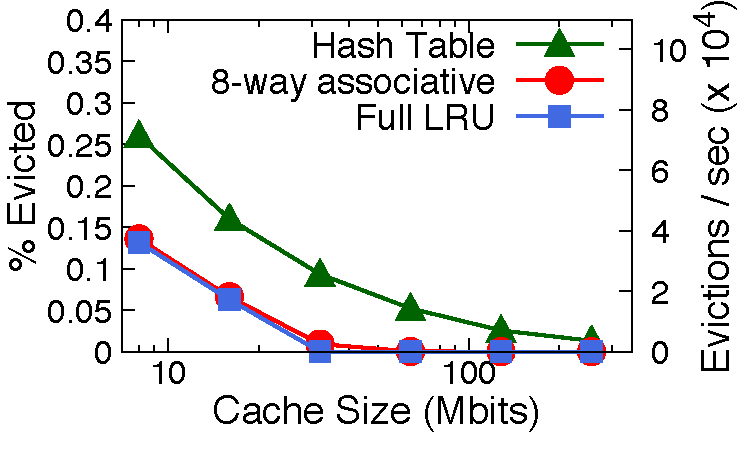
\includegraphics[width=\linewidth]{pq_eviction-rate-geo-dc.pdf}
\caption{By cache geometry (DC)}
\label{fig:eviction-geo}
\end{subfigure}
\caption{Measured eviction rates to the backing store.}
\end{figure}

The results offer three insights. First, a full LRU offers the lowest eviction
rates, since the entire LRU must be filled before an eviction occurs. However,
the 8-way associative cache comes within 2\% of this optimum, suggesting that it
is a good compromise: it avoids the hardware complexity of a full LRU without
compromising much on eviction rate. 
Second, the percentage of packets that result in an eviction at the target cache size of 32 Mbits is $\approx6\%$ for core internet switches. For the typical workload described above, this corresponds to an eviction rate of 1.67M packets per second. This is within the capabilities of multi-core scale-out key-value stores~\cite{redis_benchmark, memcached_benchmark, redis_vs_memcached, redis_vs_memcached_update}.
Third, the university datacenter setting, which is a target use case for Marple,
demands extremely little from the backing store since it has fewer unique keys
and thus fewer evictions, requiring it to sustain only 2500 packets per
second. A single processor core can handle this load. Additionally, a shorter
query that lasts only 5 minutes incurs only 3 evictions per second.

%TODO(vikram): fill in these numbers.
In context, the backing store requirements are modest. For a single ToR switch in a datacenter running at 640Gbps, a single 8-core server is sufficient to handle the eviction load. A multi-pipeline core router running at 6.4Tbps (\eg~\cite{tofino}) requires 10 such servers or 3 32-core machines. Note that the cost of these servers is low relative to the cost of the core router itself.

\Para{Accuracy of non-mergeable queries.}
Queries that are neither linear-in-state nor associative cannot be merged in the
backing store. If a key from such a query is evicted multiple times, \TheSystem
can no longer guarantee its correctness, and marks it as invalid. However, these
keys are still valid over a shorter time interval (until they are re-inserted in the
cache after an eviction). We quantify a query's accuracy as the fraction
of \emph{valid} keys over the query's lifetime. Figure~\ref{fig:accuracy-traces}
shows how query accuracy varies among the three traces, with the DC trace
near perfect since it has fewer unique keys, and hence, evictions.

If the query is run over a shorter time interval, its accuracy is typically higher, since the cache may not be full and a smaller fraction of keys are evicted. 
Figure~\ref{fig:accuracy-time} shows the tradeoff between query interval and accuracy for a variety of cache sizes and geometries using the Core16 trace.
Shortening the query from 5 minutes to 1 minute boosts accuracy by 10\%. Users running non-mergeable aggregations should consider running shorter queries to increase accuracy.

\begin{figure}[ht]
\centering
\vspace{-0.1in}
\begin{subfigure}[t]{0.48\columnwidth}
\raggedright
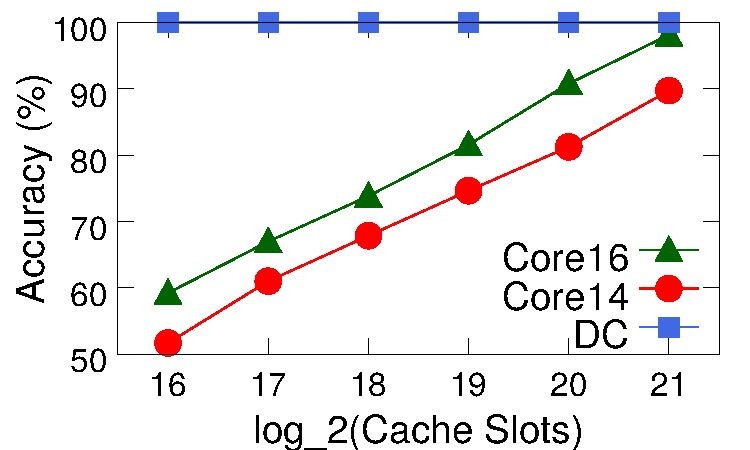
\includegraphics[width=\linewidth]{pq_accuracy-alltraces.pdf}
\caption{By trace}
\label{fig:accuracy-traces}
\end{subfigure}
\begin{subfigure}[t]{0.48\columnwidth}
\raggedleft
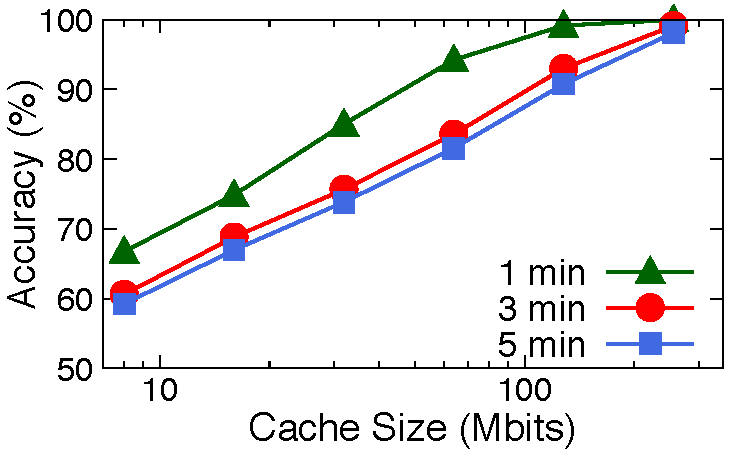
\includegraphics[width=\linewidth]{pq_accuracy-core-geo.pdf}
\caption{By cache geometry (Core16)}
\label{fig:accuracy-time}
\end{subfigure}
\caption{Query accuracy for non-mergeable aggregations.}
\end{figure}


\subsection{Debugging case study with Mininet}
\label{s:eval:mininet}
\label{sec:eval:mininet}


To demonstrate \TheSystem's use in practice, we present a case study using
Mininet~\cite{mininet}.
%with a topology shown in Figure~\ref{fig:mininet-topo}.
Our topology consists of 4 hosts ({\ct h1, h2, h3, h4}) and 2 switches in a dumbbell topology.
One switch is connected to {\ct h1} and {\ct h3}
and the other, to {\ct h2} and {\ct h4}.
The switches are connected via a single link and
programmed in \pfs~\cite{p4-bmv2} with queries compiled by \TheSystem.

Host {\ct h2} repeatedly downloads a 1MB objects over TCP from {\ct h1}.
Meanwhile, {\ct h3} sends {\ct h4} sporadic bursts of UDP traffic, which
{\ct h4} acks.  Suppose a network admin notices the irregular latency
spikes for the TCP traffic (\Fig{mininet-latency}). She suspects a queue buildup
in the switches and measures the queue depths seen by the traffic by writing:
{\ct result = filter(\pktlog, srcip == h1 and dstip == h2).}

% Can remove this figure if we need space.
%\begin{figure}[ht]
%\centering
%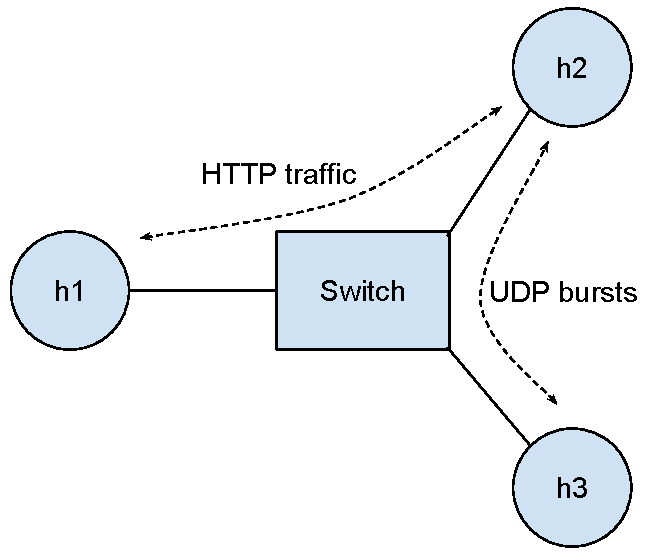
\includegraphics[width=0.4\columnwidth]{mininet-topo.pdf}
%\caption{Mininet topology used for the case study.}
%\label{fig:mininet-topo}
%\end{figure}

\begin{figure}[!t]
\centering
\vspace{-0.1in}
\begin{subfigure}[t]{0.48\columnwidth}
\raggedright
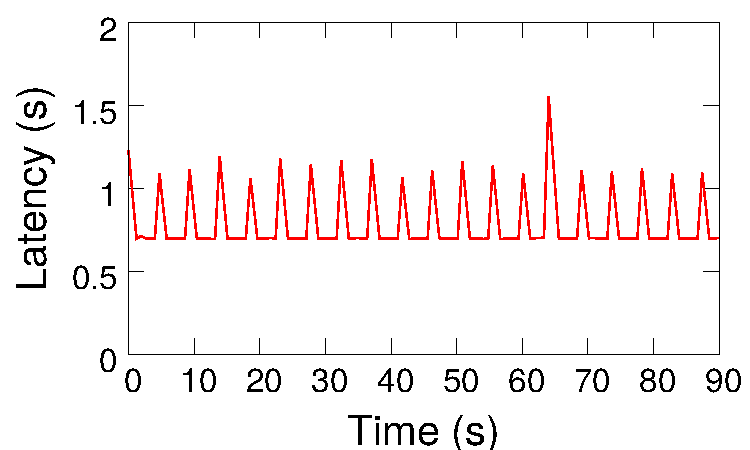
\includegraphics[width=\linewidth]{pq_fetch_latency.pdf}
\vspace{-0.2in}
\caption{TCP request latency}
\label{fig:mininet-latency}
\end{subfigure}
\begin{subfigure}[t]{0.48\columnwidth}
\raggedleft
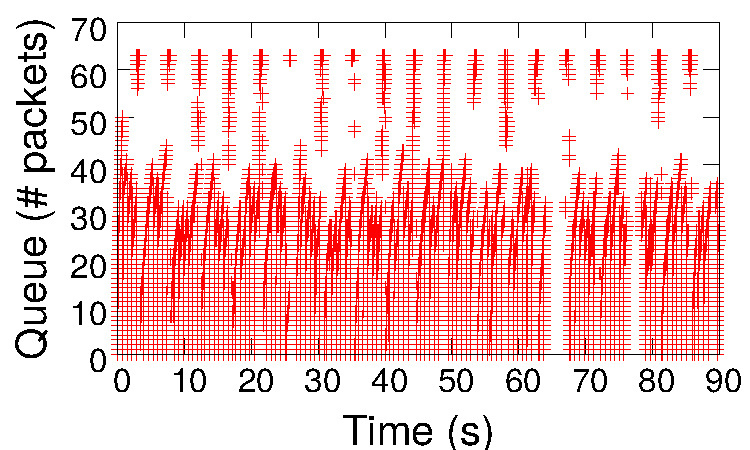
\includegraphics[width=\linewidth]{pq_queue_sizes.pdf}
\vspace{-0.2in}
\caption{Queue depth at egress port 2}
\label{fig:mininet-qin}
\end{subfigure}
\vspace{0.05in}
\caption{Mininet case study measurements.}
\end{figure}
\begin{table}[t]
\centering
\small
\begin{tabular}{|c|c|c|c|c|} \hline
\bf{src $\rightarrow$ dst} & \bf{protocol} & \bf{\# Bursts} & \bf{Time ($\mu$s)} & \bf{\# Packets} \\ \hline
h3:34573 $\rightarrow$ h4:4888 & UDP & 19 & 8969085 & 6090 \\
h4:4888 $\rightarrow$ h3:34573 & UDP & 18 & 10558176 & 5820 \\
h1:1777 $\rightarrow$ h2:58439 & TCP & 1 & 72196926 & 61584 \\
h2:58439 $\rightarrow$ h1:1777 & TCP & 1 & 72248749 & 33074 \\ \hline
\end{tabular}
\caption{Per-flow burst statistics from \TheSystem.}
\label{t:mininet-flowstats}
\vspace{-0.1in}
\end{table}

The results are streamed out on each packet to a collection server. After
plotting the queue latencies, she notices spikes in queue size at egress port 3
on the switch (\Fig{mininet-qin}) matching the periodicity of the latency
spikes. To isolate the responsible flow(s), she divides the traffic into
``bursts'', which she defines as a series of packets separated by a gap of at
least 800ms, as determined from the gap between latency spikes. She issues the
following \TheSystem query:

\begin{small}
\begin{lstlisting}
def burst_stats(last_time, nburst, time, pkts, tin):
    if tin - last_time > 800000:
        nbursts++;
        emit();
    else:
        time = time + tin - last_time;
    pkts = pkts + 1;
    last_time = tin;
result = groupby(R1, (*\codeftuple{}*), burst_stats)
\end{lstlisting}
\end{small}

%% NG->Vikram: The burst table is moved to related work to bring it to the head
%% of the next column.

%%\vspace{-0.1in}
She runs the query for 72 seconds and sees the result in
Table~\ref{t:mininet-flowstats}. She concludes, correctly, that UDP traffic
between {\ct h3} and {\ct h4} is responsible for the latency spikes.
There are 18 UDP bursts, with an average size of 320 packets and
average duration of 472 ms, which matches our emulation setup.

\TheSystem's power and flexibility make this diagnosis simple. End host solutions
 are blind to queue contention on the switch, and flexible
aggregations expose flow statistics customized for the problem:
packet counts alone would have disguised the bursty nature of
the offending UDP traffic.



%\subsection{[Reach] Redis benchmarking}

%% % Maybe have a list of questions we want to answer to motivate this section
%% % such as FSCQ, section 7 at SOSP15.
%% \subsection{Expressiveness}
%% % TODO: Table for this.
%% % Which queries can be expressed?
%% % Which are linear in state?

%% \subsection{Hardware resources for running queries}
%% % TODO: Write a script for this.
%% % What's the pipeline depth and width?
%% % What atoms beyond linear-in-state are required?

%% \subsection{What is the memory requirement?}
%% % TODO: Write a script for this.
%% % Run trace-driven simulations on CAIDA + Theo Benson's traces.
%% % Maybe run on FB data as well?
%% % Show how linear-in-state significantly reduces memory requirement.
%% % Alternatively show how it reduces load on the backend server.

%% \subsection{How much traffic does the backend server need to process?}

%% % Bombard REDIS with transactions from our corpus at a certain rate.
%% % See how many servers we need to process these transactions.
%% % Exploit the fact that transaction latency can be high so long as transaction throughput is high

%% \subsection{How many servers does this cost in total?}

%% % Get some back of the envelope numbers based on level of aggregation, typical query, REDIS results, exact query etc.
%% % Want a bottomline number like: for x% additional servers, we can have these useful measurement abilities.
%% % Maybe elevate to introduction.

%% \subsection{Mininet evaluations}

%% % ex1: TCP client, server.
%% % UDP workload
%% % Latency spike

%% % ex2: flowlet size histogram

%% % ex3: how long is a high prio packet blocked because a low prio is currently in transmission?

%% % show graphs for each one of these scenarios.
